\subsection{Symptomer}
KOL udvikles over mange år, dog bemærkes sygdommen ofte ikke før lungefunktionen er markant nedsat. Dette betyder, at KOL og dens symptomer som regel først kommer til udtryk efter $50$ årsalderen\cite{Lange2015}. Dette kan betyde, at patienter først opsøger en læge, når deres lungefunktion er halveret \cite{dsam2016}.

Symptomer på KOL opleves som åndenød og hoste ved fysisk aktivitet. Hosten er ofte med ekspektoration, som hos de fleste patienter er klart eller hvidt.\cite{Basisbogen2016} Derudover er der en tendens til hyppig eksacerbationer, hvilket er tilfælde, hvor KOL-patienters tilstand forværres akut og kræver behandling. Symptomerne hertil opleves som øget åndenød, hoste samt grønt eller gulligt ekspektoration og øget purulens. Denne tilstand skyldes ofte infektioner med bakterier, hvilket udgør ca. 50 \% af tilfældene.\cite{Basisbogen2016, dsam2016} 

Der er en række komorbiditeter, som hyppigt ses hos KOL-patienter, som desuden kan have en negativ påvirkning på patienters livskvalitet og prognose. Derfor bør patienter regelmæssigt tjekkes for de hyppigste komormiditeter, såsom kardiovaskulære sygdomme, type-2 diabetes, osteoporose, lungecancer, muskelsvækkelse samt angst og depression.
Nogle af komorbiditeterne kan skyldes, at åndenød har medført et nedsat fysisk aktivitetsniveau og dermed svage perifere muskler samt vægttab. Desuden har tobakrygning og generelt dårlig livsstil ligeledes betydning for udviklingen af disse komorbiditeter. \cite{dsam2016, McCarthy2015}
Psykiske komorbiditeter, ofte i form af depression og angst, har en øget forekomst hos patienter med en FEV1 værdi på under 50 \% af den forventede værdi. Den øgede risiko for psykiske lidelser skyldes, at KOL kan medføre social isolation og tab af sociale relationer, skyldfølelse, usikkerhed i forhold til fremtiden. \cite{dsam2016}


\subsection{Diagnose}
Ved mistanke om KOL undersøges lungefunktionen ved spirometriundersøgelser, hvor FEV1 og FVC måles. Af \autoref{fig:FEV} ses spirometrimålinger for henholdsvis patienter med normal, obstruktiv og restriktiv nedsat lungefunktion samt en kombination af disse.\cite{Basisbogen2016, Sundhed2013}

\begin{figure} [H]
\centering
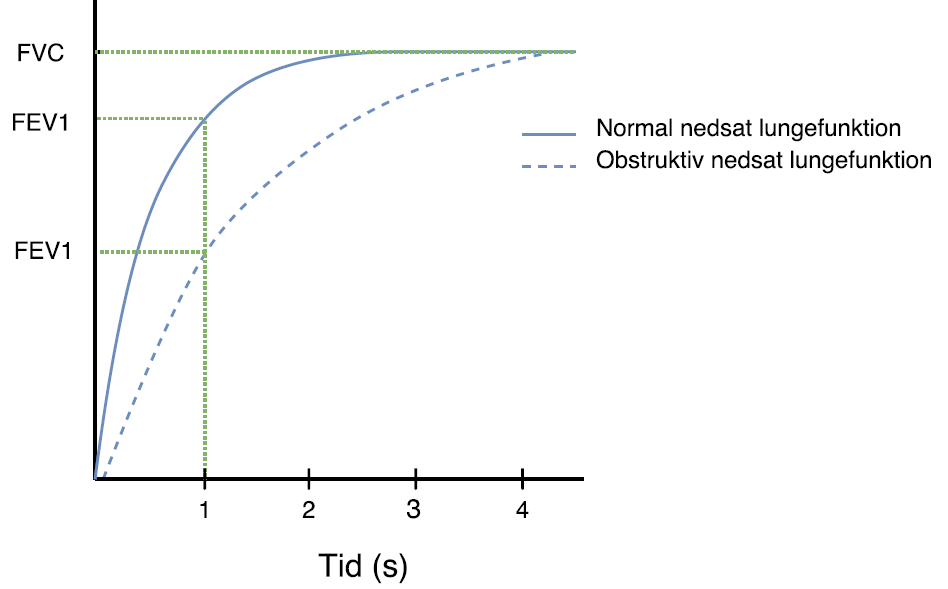
\includegraphics[width=0.5\textwidth]{figures/FEV}
\caption{Spirometrimålinger for patienter med normal, obstruktivt og restriktiv nedsat lungefunktion samt patienter med kombineret obstruktivt og restriktivt nedsat lungefunktion.}
\label{fig:FEV}
\end{figure} 

\noindent
Det fremgår af \autoref{fig:FEV}, at der ved obstruktivt og restriktiv nedsat lungefunktion er et fald i FEV1 samt lungefunktionen. Der udføres desuden en reversibilitetstest for at sikre, at patienten ikke lider af differentialdiagnosen astma. Disse patienter gives broncodilatorer, som hos astmapatienter vil forbedre spirometrimålingen, mens lungefunktionen for KOL-patienter forbliver uændret.\cite{Basisbogen2016, Sundhed2013} 
For at undersøge KOL og komobiditeter, som er forbundet med KOL undersøges foruden lungefunktionsundersøgelser BMI, røntgen af thorax, EKG-målinger og blodprøver \cite{Sundhed2013}. 
%Med tiden kan symptomerne på KOL forværres, og der skal mindre fysisk aktivitet til for at udløse åndenød. \cite{Basisbogen2016}